\section*{Características del móvil HTC Desire}
\addcontentsline{toc}{chapter}{Características del móvil HTC Desire}
En Enero de 2010 la compañia HTC saca al mercado un nuevo smartphone, en él se ejecuta la versión 2.2 del sistema operativo Android. El desarrollo del proyecto se ha centrado en este móvil debido a que es uno de los primeros móviles con un procesador Snapdragon de 1Ghz, que contiene un chipset gráfico Adreno 200, soportando la programación de la GPU (unidad de procesamiento gráfico) mediante la inclusión de shaders.
\newline 

\begin{center}
\begin{tabular}{|l|l|}
\hline
\rowcolor[gray]{.8}Característica & Descripción \\\hline
\hline
Dimensiones  			& 119 x 60 x 11,9 milímetros						\\\hline
Peso				 	& 135 gramos 								 	\\\hline
Procesador			& Procesador Qualcomm Snapdragon a 1 GHz			\\\hline
Chipset gráfico			& Adreno 200 con soporte OpenGL ES 2.0				\\\hline
Memoria RAM	 		& 576MB 										\\\hline
Memoria ROM  			& 512MB	hasta 32GB							\\\hline
Pantalla		 		& AMOLED multitáctil de 3.7 pulgadas					\\\hline
Resolución	 			& WVGA (480 x 800 píxeles)						\\\hline
Cámara			 	& 5MB										\\\hline
Vídeo				& Alta definición 720p								\\\hline
Batería			 	& 1400 mAh 									\\\hline
Red					& SPA/WCDMA y MHz y GSM						\\\hline
Conectividad			& 3G, GPRS, EDGE y WiFi (802.11b/g)					\\\hline
Autonomía	3G 			& 360 horas en espera y 6 horas 30 minutos  			\\\hline
Bluetooth				& Con soporte A2DP								\\\hline
GPS 					& Con soporte A-GPS								\\\hline
Radio				& Sí											\\\hline
Jack 3.5mm			& Sí											\\\hline
Micro USB				& Sí											\\\hline
Acelerómetro			& Sí											\\\hline
Brújula digital 			& Sí											\\\hline
Sensor de proximidad 	& Sí											\\\hline
Sensor de luz ambiental 	& Sí											\\\hline
Puerto inflarojos			& No											\\\hline
\end{tabular}
\end{center}

\begin{figure}[h]
	\centering	
         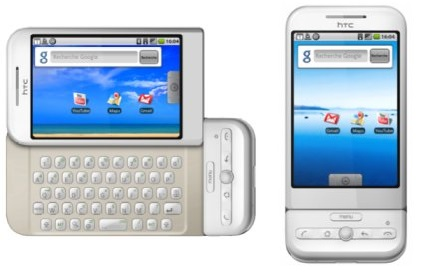
\includegraphics[height=90mm]{img/htc-dream.jpg}
	\caption{Dispositivo móvil HTC Dream}
\end{figure}

\begin{figure}[h]
	\centering	
         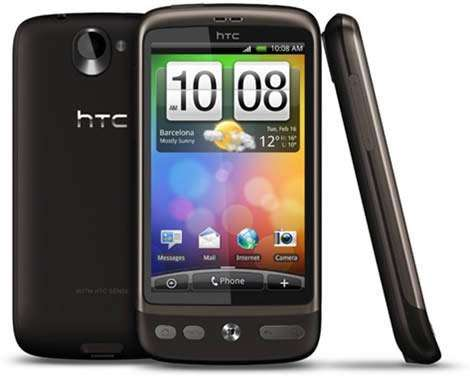
\includegraphics[height=90mm]{img/htc-desire.jpg}
	\caption{Dispositivo móvil HTC Desire}
\end{figure}


